% https://sites.google.com/vols.utk.edu/rewords23/home
\PassOptionsToPackage{hyphens}{url}
\documentclass[conference]{IEEEtran}
\IEEEoverridecommandlockouts

% The preceding line is only needed to identify funding in the first footnote. If that is unneeded, please comment it out.

\usepackage{cite}
\usepackage{amsmath,amssymb,amsfonts}
\usepackage{algorithmic}
\usepackage{graphicx}
\usepackage{textcomp}
\usepackage[dvipsnames]{xcolor}
\usepackage{comment}
\usepackage[hidelinks]{hyperref}
\usepackage{fancyvrb}
\usepackage{fvextra}

\PassOptionsToPackage{hyphens}{url}
\pdfoutput=1

\usepackage[pdf]{graphviz}

\usepackage{fancyvrb}
\usepackage{todonotes}
\newcommand{\TODO}[1]{\todo[inline]{#1}}
\newcommand{\NOTE}[1]{\textcolor{red}{[NOTE: #1]}}
%\newcommand{\FILE}[1]{\todo[inline,color=green!20]{File: #1}}
\newcommand{\FILE}[1]{}

\renewcommand\IEEEkeywordsname{Keywords}
\newcommand{\orcidicon}[1]{\href{https://orcid.org/#1}{
\includegraphics[width=9pt]{orcid_icon}}}

% \usepackage{color}
\usepackage{listings}
% \usepackage{xcolor}
% \usemintedstyle{trac}
% \definecolor{mblue}{rgb}{0.27,0.33,0.53}

\lstset{
  basicstyle=\scriptsize\ttfamily,
  breaklines=true,
  keywordstyle=\color{BrickRed},
  moredelim=[s][\color{BrickRed}]{\{}{\}},
  % moredelim=[s][\bfseries]{workflow:}{\n},
  % moredelim=[s][\bfseries]{nodes:}{\n},
  % literate={\{}{{\textbf{\{}}}1
  % literate={workflow:}{{{\bfseries workflow:}}}9,
  % literate={nodes:}{{{\bfseries nodes:}}}6,
  escapeinside={(*}{*)}
}

% these do not use shell escape!
% therefore they are arxiv safe

\lstdefinestyle{python}{
  language=Python,
  basicstyle=\scriptsize\ttfamily,
  keywordstyle=\color{blue},
  commentstyle=\color{green!50!black},
  stringstyle=\color{Bittersweet},
  showstringspaces=false,
  breaklines=true
}

\lstdefinestyle{sh}{
  language=sh,
  basicstyle=\scriptsize\ttfamily,
  keywordstyle=\color{blue},
  commentstyle=\color{green!50!black},
  stringstyle=\color{Bittersweet},
  showstringspaces=false,
  breaklines=true,
  keywords={singularity,echo}
}

% \lstdefinestyle{yaml}{
%   keywordstyle=\bfseries\color{blue},
%   moredelim=[s][\bfseries\color{blue}]{workflow:}{\n},
%   moredelim=[s][\bfseries\color{blue}]{nodes:}{\n}
% }

\definecolor{friendlybg}{HTML}{f0f0f0}
\definecolor{lightgray}{rgb}{.9,.9,.9}
\definecolor{darkgray}{rgb}{.4,.4,.4}
\definecolor{purple}{rgb}{0.65, 0.12, 0.82}

    
\begin{document}

\title{Hybrid Reusable Computational Analytics Workflow Management with Cloudmesh Applied to the MLCommons Cloudmask Application\thanks{Funded by NSF, DOE, NIST, and University of Virginia. In part funded by the NSF CyberTraining: CIC:
CyberTraining for Students and Technologies from Generation Z with the
award numbers 1829704 and 2200409 and NIST 60NANB21D151T.}
}
  
\author{\IEEEauthorblockN{1\textsuperscript{st} Gregor von Laszewski}
\IEEEauthorblockA{\textit{Biocomplexity Institute}\\
\textit{University of Virginia}\\
Charlottesville, VA 22911, USA \\
laszewski@gmail.com \\
0000-0001-9558-179X}
\and
\IEEEauthorblockN{2\textsuperscript{nd} J.P. Fleischer}
\IEEEauthorblockA{\textit{Biocomplexity Institute}\\
\textit{University of Virginia}\\
Charlottesville, VA 22911, USA \\
jacquespfleischer@gmail.com \\
0000-0002-1102-1910}
\and
\IEEEauthorblockN{3\textsuperscript{rd} Geoffrey C. Fox}
\IEEEauthorblockA{\textit{Biocomplexity Institute}\\
\textit{University of Virginia}\\
Charlottesville, VA, USA \\
gcfexchange@gmail.com \\
0000-0003-1017-1391}
\and
\IEEEauthorblockN{4\textsuperscript{th} Juri Papay\\
5\textsuperscript{th} Sam Jackson}
\IEEEauthorblockA{\textit{Rutherford Appleton Laboratory}\\
Harwell Campus\\
Didcot, OX11 0QX, UK}
}
% samuel.jackson@stfc.ac.uk 



\maketitle
% -------------------------------
% remove this for no page numbers
\thispagestyle{plain}
\pagestyle{plain}
% -------------------------------

\begin{abstract}

 In this paper, we summarize our effort to create and utilize a {\em
 simple} framework to coordinate computational AI analytics tasks with
 the help of a workflow system. Our design is based on a minimalistic
 approach while at the same time allowing access to hybrid
 computational resources offered through the owner's computer, HPC
 computing centers, cloud resources, and distributed systems in
 general. Access to this framework includes a simple GUI for
 monitoring and managing the workflow, a REST service, a command line
 interface, as well as a Python interface. It also includes a template
 based batch management system that, through configuration files, easily allows 
 for the generation of reproducible experiments while creating permutations over
 selected experiment parameters as typical in deep learning applications. The resulting framework was
 developed for analytics workflows targeting benchmarks of AI
 applications on hybrid computing resources, as well as an educational tool
 for teaching scientists and students sophisticated concepts to
 execute computations on resources ranging from a single computer to
 many thousands of computers as part of on-premise and cloud
 infrastructure. We demonstrate the usefulness of the tool while
 creating FAIR principle-based result generation for the MLCommons
 Science Working Group Cloudmask application. The code is available as
 an open-source project in GitHub and is based on an easy-to-enhance
 tool called Cloudmesh.


\end{abstract}

\begin{IEEEkeywords}
experiment workflow, task workflow, high performance computing, batch queue, workflow web service
\end{IEEEkeywords}

% \section{Introduction}




%\renewcommand{\shortauthors}{von Laszewski, et al.}



% 
\begin{CCSXML}
<ccs2012>
<concept>
<concept_id>10010520.10010521.10010537</concept_id>
<concept_desc>Computer systems organization~Distributed architectures</concept_desc>
<concept_significance>500</concept_significance>
</concept>
<concept>
<concept_id>10010520.10010521.10010537.10003100</concept_id>
<concept_desc>Computer systems organization~Cloud computing</concept_desc>
<concept_significance>500</concept_significance>
</concept>
<concept>
<concept_id>10011007.10010940.10010971.10011120</concept_id>
<concept_desc>Software and its engineering~Distributed systems organizing principles</concept_desc>
<concept_significance>500</concept_significance>
</concept>
</ccs2012>
\end{CCSXML}

\ccsdesc[500]{Computer systems organization~Distributed architectures}
\ccsdesc[500]{Computer systems organization~Cloud computing}
\ccsdesc[500]{Software and its engineering~Distributed systems organizing principles}

\keywords{high performance computing, batch queue, service}




%\begin{CCSXML}
%<ccs2012>
%<concept>
%<concept_id>10010520.10010521.10010537</concept_id>
%<concept_desc>Computer systems organization~Distributed architectures</concept_desc>
%<concept_significance>500</concept_significance>
%</concept>
%<concept>
%<concept_id>10010520.10010521.10010537.10003100</concept_id>
%<concept_desc>Computer systems organization~Cloud computing</concept_desc>
%<concept_significance>500</concept_significance>
%</concept>
%<concept>
%<concept_id>10011007.10010940.10010971.10011120</concept_id>
%<concept_desc>Software and its engineering~Distributed systems organizing principles</concept_desc>
%<concept_significance>500</concept_significance>
%</concept>
%</ccs2012>
%\end{CCSXML}

%\ccsdesc[500]{Computer systems organization~Distributed architectures}
%\ccsdesc[500]{Computer systems organization~Cloud computing}
%\ccsdesc[500]{Software and its engineering~Distributed systems organizing principles}

% \keywords{high performance computing, batch queue, service}



%\received{20 February 2007}
%\received[revised]{12 March 2009}
%\received[accepted]{5 June 2009}

% set page numbers
% \settopmatter{printfolios=true}

\maketitle

% \FILE{cc.tex}

\section{Introduction}

In this section we provide an introduction to our work while
moving forward to motivate a 
Hybrid Reusable Computational Analytics Workflow
Management Framework.

\subsection{Reusable Computational Analytics}

{\em Reusable computational analytics} (RCA) focuses on the creation of reusable programs, patterns, and services to conduct analytics tasks that are part of the scientific discovery process. RCA service need varies widely and may include multi-scale hardware resources as well as multi-scale scientific applications. To utilize such services and their resources in a reusable way, we need to have a mechanism to express them in an easy fashion that goes beyond just the definition in one programming language or framework, but allows the integration into many different programming languages and frameworks so that services that may be designed in one framework or language may be reusable in others.

\subsection{Reusable Multi-scale Algorithms}

In current scientific problems we encounter a rich set of applications that leverage a number of sophisticated methods that may require adaptations on multiple scales. The scales are influenced by their Domain size, accuracy and time requirement to solve them in a sufficient manner. It is of advantage to provide reusable components that can be controlled by parameters to simplify reuse.

\subsection{Hybrid Cloud and Compute Resources and Serices}

As we deal with multi-scale algorithms, not every analytics task needs to be conducted on a High Performance Computer (HPC). This is especially the case with the advent of desktop GPUs, which authors have termed in past {\em desktop supercomputing}. Also the availability of cloud computers and hyper-scale data centers play a significant role in today's analytics processes. This not only includes the use compute resources, but also services that are these days offered by cloud service providers. A well-known example for this is natural language processing.

\subsection{Reusable and Adaptable HPC and Cloud Service Workflows}

High-performance computing (HPC) has been, for decades, a very important tool
for science. Scientific tasks can leverage the processing power of
a supercomputer so they can run at previously unobtainable high speeds
or utilize specialized hardware for acceleration that otherwise are not
available to the user. HPC can be used for analytic programs that
leverage machine learning applied to large data sets to, for example,
predict future values or to model current states. For such
high-complexity projects, there are often multiple complex programs that
may be running repeatedly in either competition or cooperation.
Leveraging computational GPUs, for instance, leads to several times higher
performance when applied to deep learning algorithms. With such
projects, program execution is submitted as a job to a typically remote
HPC center, where time is billed as node hours. Such projects must have
a service that lets the user manage and execute without supervision. We
have created a service that lets the user run jobs across multiple
platforms in a dynamic queue with visualization and data storage.

Similar aspects are available for cloud services that abstract the infrastructure needs and focus on the availability of services that can be integrated in concert with HPC, as well as the users local resources (for example a PC).




\FILE{cc.tex}

\section{Introduction}

In this section, we provide an introduction to our work while
moving forward to motivate a 
Hybrid Reusable Computational Analytics Workflow
Management Framework.

Our long-term involvement as part of the MLCommons Science Working Group has greatly influenced this work. MLCommons is a non-profit organization that brings together over 70 members from industry, academia, and government, with the aim of accelerating machine learning innovation for the benefit of all~\cite{www-mlcommons}. One of its primary objectives is to develop standardized benchmarks for assessing the performance of machine learning systems and applying them to various applications.
These applications encompass a wide range of domains, including healthcare, automotive, image analysis, and natural language processing, among others. MLCommons focuses on benchmarking training~\cite{mlperf-training} and validation algorithms to track progress over time. To achieve this goal, MLCommons explores machine learning efforts in the realms of benchmarking, dataset development for benchmarking purposes, and the establishment of best practices that make effective use of machine learning. MLCommons is organized into several working groups that tackle specific topics, such as benchmarking in relation to training, training on high-performance computing (HPC) resources, and inference performed on data centers, edge devices, mobile devices, and embedded systems. Best practices are investigated in areas such as infrastructure and power management. Moreover, MLCommons operates additional working groups dedicated to Algorithms, DataPerf Dynabench, Medical, Science, and Storage.

The Science Working Group within MLCommons is primarily focused on advancing the scientific aspects beyond the mere creation of static benchmarks \cite{las-22-mlcommons-science}. The work presented here is an outcome of our contributions to the goals set forth by the MLCommons Science Working Group.

As part of this activity, we are collaborating with a large number of researchers, including aspiring researchers from various academic institutions. However, we are confronted with multiple challenges:
(a) Many participants are not sufficiently familiar with using high-performance computing (HPC) or other resources to conduct reproducible experiments reliably.
(b) When dealing with different compute resources, special system configurations need to be developed for each resource, and these configurations may even vary from user to user on the system.
(c) Creating a reproducible experiment is often out of scope as the focus for beginning students that may not have the time to run and understand the application during a semester activity.

What we strive to achieve is to make the situation simpler for the students while working at the same time towards the implementation of the FAIR principle \cite{www-fair} for the targeted MLCommons Science applications addressing the previously mentioned issues. 

Although we are applying our approach to other applications, we focus here on the MLCommons Cloudmask \cite{las-22-mlcommons-science} application that tries to identify the cloud cover from satellite images.

The paper is structured as follows. First, we discuss the important requirement aspects that influenced the design and implementation of our work in Section \ref{sec:requirements}. We then provide an overview of related research in Section \ref{sec:related-research}. Next, we present the design of the workflow framework in Section~\ref{sec:design}. To demonstrate the practical use of the framework, we showcase its capabilities to specify task-based workflows in Section \ref{sec:task-workflow}, followed by a detailed discussion on how to interface with the workflows in Section \ref{sec:cloudmesh-cc-interfaces}. Additionally, we briefly outline other notable cloudmesh features in Section \ref{sec:cloudmesh-other}. Furthermore, we illustrate how cloudmesh can effectively coordinate hyperparameter-based workflows for the cloudmask application in Section \ref{sec:cloudmask-workflow}. Finally, we conclude our paper in Section \ref{sec:conclusion}.


\section{Requirements}
\label{sec:requirements}

We list the requirements that influence our design and describe in more detail requirements arising from reusability, design, and implementation-specific requirements.

\subsection{Reusability Requirements}

\subsubsection{Reusable Computational Analytics}

Reusable computational analytics (RCA) focuses on the creation
of reusable programs, patterns, and services to conduct analytics
tasks that are part of the scientific discovery process. The need for
RCA is vast and may include multi-scale hardware resources as
well as multi-scale scientific applications. To utilize such services
and their resources in a reusable way, we need to have a mechanism to
express them in an easy fashion that goes beyond just the definition
in one programming language or framework, and allows the integration
into many different programming languages and frameworks so that
services that may be designed in one language or framework may be
reusable in others.

\subsubsection{Reusable Multi-scale Algorithms}

In current scientific problems, we encounter a rich set of applications
that leverage a number of sophisticated methods that may require
adaptations on multiple scales. The scales are influenced by their
domain size, accuracy, and time requirement to solve them adequately. It is advantageous to provide reusable components
that can be controlled by parameters to simplify reuse.


\subsubsection{Hybrid Cloud and Compute Resources and Serices}

As we deal with multi-scale algorithms, not every analytics task needs
to be conducted on a High-Performance Computer (HPC). This is
especially the case with the advent of desktop GPUs, which authors
have termed in the past {\em desktop supercomputing}. Also, the
availability of cloud computers and hyper-scale data centers plays a
significant role in today's analytics processes. This not only
includes the use of computing resources but also services that are 
offered by cloud service providers. A well-known example of this
is natural language processing.

\subsubsection{Reusable and Adaptable HPC and Cloud Service Workflows}

High-performance computing (HPC) has been, for decades, a very important tool
for science. Scientific tasks can leverage the processing power of
a supercomputer so they can run at previously unobtainable high speeds
or utilize specialized hardware for acceleration that otherwise are not
available to the user. HPC can be used for analytic programs that
leverage machine learning applied to large data sets to, for example,
predict future values or to model current states. For such
high-complexity projects, there are often multiple complex programs that
may be running repeatedly in either competition or cooperation.
Leveraging computational GPUs, for instance, leads to several times higher
performance when applied to deep learning algorithms. With such
projects, program execution is submitted as a job to a typically remote
HPC center, where time is billed as node hours. Such projects must have
a service that lets the user manage and execute without supervision. 
Therefore, we have created a service that lets the user run jobs across multiple
platforms in a dynamic queue with visualization and data storage.

Similar aspects are available for cloud services that abstract the
infrastructure needs and focus on the availability of services that
can be integrated in concert with HPC, as well as the user's local
resources (a PC, for example).

\subsection{Design and Implementation Requirements}

For the design of the framework, we have the following requirements.

\subsubsection{Simplicity}

The design must be simple and the code base must be
small. This not only helps future maintenance of the code, but also allows
the code to become part of educational opportunities such as in a
Research Experience for Undergraduates (REU), capstone project, and
class projects. The challenge here is that many other systems are too
big to be used in introductory undergraduate and master's activities.
However, the framework should be capable enough to also support
research projects.

\subsubsection{Workflow Specification} The specification of the workflow must
be simple. In the past, we have learned that the introduction of
programming control components, such as loops and conditions, in
addition to DAGs, is essential to provide maximum flexibility.

\subsubsection{Workflow Monitoring} The workflow framework must be able to
monitor the progress of individual jobs as well as the overall
progress of the workflow.

\subsubsection{Workflow Interfaces} To specify and interface with the
workflow, we must provide several interface layers. This includes
specification through a YAML file, interfacing through REST calls,
interfacing through a Python API, and interfacing with a very simple
GUI component. For the workflow monitoring with the GUI, we must be
able to easily define custom text to reflect user-designable
monitoring labels.

\subsubsection{Language Independence} As we want to make the framework
integratable into other frameworks, we need a simple mechanism to provide
either API or interface portability. To keep the code base small, a
REST API seems very well-suited.

\subsubsection{OpenAPI} To further strengthen usability, the framework must
have an OpenAPI interface. This allows the integration via 3rd party
tools into other frameworks and languages if desired.

\subsubsection{Hybrid Multicloud Providers} The service must be able to be
deployable on an on-premise local computer or various cloud providers.

\subsubsection{Generalized Job Interface} The framework must be able to
interface with a wide variety of computation services. This includes
the support of ssh, batch queues such as SLURM \cite{www-slurm} and
LSF \cite{www-lsf}, and local
compute resources including shell scripts, as well as support for WSL.

\subsubsection{Support of Various Operating Systems} The framework must be
runnable on various client operating systems including Linux, macOS, and
Windows.

\subsubsection{State Management} The state management must be recoverable and
the client must be able to completely recover from a network failure.
As such, the state will be queried on demand. This allows one to
deploy the framework on a laptop, start the workflow, close or
shutdown the laptop, and at a later time open the laptop while the
workflow framework can be refreshed with the latest state.


\section{Related Research}
\label{sec:related-research}

Many different workflow systems have been developed in the past. It is
out of the scope of this document to present a complete overview of
all the different systems. Instead, we list some of the systems and organize them in various categories within this section. A more detailed analysis is available
at \cite{las-22-arxiv-workflow-cc}. One of the systems that have been developed is MLCube \cite{www-mlcube} which is developed within MLCommons. Similar to our framework, it uses YAML specification for organizing, running, and sharing machine learning experiments. It attempts to standardize the 
 format for defining and packaging machine learning projects, including their code, dependencies, datasets, and configurations. Through this, it aims to 
 facilitate the reproducibility and portability of machine learning experiments by encapsulating all the necessary components in a self-contained and portable container. Our system is needed as it provides both an enhancement on top of MLCube, as well as on the bottom.
 Thus, we could integrate tools and services we developed within an MLCube specification, but also use MLCube within our framework. One of the features we try to emphasize is that we do not distribute a container in general, but just the description of how the container can be created either in Docker or Singularity. This is important when the customization of the experiment and its applications is in the foreground. Furthermore, at the time of writing, the support of MLCube for Singularity was not supporting our locally available resources (on which Docker is not supported) so we could not utilize it. As a result, our team has proposed changes to MLCube that will eventually result in a usable Singularity port. 
 
Next, we list the various categories of related workflow systems while augmenting them with references. By no means is this list complete; it represents a selected number of efforts. 

\subsubsection{Batch parallelism} Long-running jobs on HPC systems are coordinated through
Batch services  \cite{www-lsf,www-slurm,www-cloudmesh-manual,www-airflow,las-1996-thesis,las-1999-loosely}.

\subsubsection{Task parallelism} Tasks are a logical unit of work that is
executed by a resource, service, or component. Task parallelism
is often used in distributed resource frameworks \cite{www-cloudmesh-manual,www-airflow,www-pegasus}.

\subsubsection{Resource Reservation} In some cases, access to batch queues on
HPC systems takes a long time. In the case of many different tasks, it
is sometimes useful to reserve a number of batch nodes and run many
short-running programs on them if the need arises. This, however, can
often be replaced just by properly coordinated workflows using a
batch system. In fact, frameworks using such reservations internally
implement them using the batch system \cite{las-02-infogram,www-pegasus,www-parsl,arxiv-radical-pilot,www-slurm}.

\subsubsection{Computational Grids} Grids provide service-level access to
distributed HPC computing resources. However, Grids (popular a decade
ago) are no longer predominantly deployed and the focus has shifted to
Cloud computing \cite{www-pegasus} as well as hyperscale HPC deployments.

\subsubsection{Cloud} Presently, computing resources are also available in
the cloud as HPC, batch, and compute services, including specialized
SaaS offerings that allow integrating analytics functions into
workflows \cite{www-cloudmesh-manual,www-airflow,www-gcloud,www-azure-rest,www-aws-workflow,www-azure-batch}.

\subsubsection{REST} The predominant specification for cloud services using the
REST framework relies on a stateless model. This contrasts with the
WSRF model that uses stateful services \cite{www-business-rest-ibm}.

\subsubsection{Specification} Some work has also focused on the specification
of the workflows  \cite{www-snakemake,las-2004-gridant,www-pegasus,las-2007-swift,www-aws-swf}.

\subsubsection{GUI} Some frameworks provide extensive GUIs \cite{www-kepler,www-aws-stepfunctions,www-azure-batch,www-azure-enterprise-workflow}.


\section{Design}
\label{sec:design}

To fulfill our requirements, we have developed a framework for
workflow-controlled computing called Cloudmesh Compute Cluster,
otherwise referred to as {\em cloudmesh-cc}. It is enhanced by a
specialized experiment executor, allowing to easily specify parameter-enhanced workflow specifications. The architecture of the
framework is depicted in Figure~\ref{fig:arch}.

\begin{figure}[htb]
% figure is somewhat off-center so nudging it to the right - JPF
\hspace{5px}
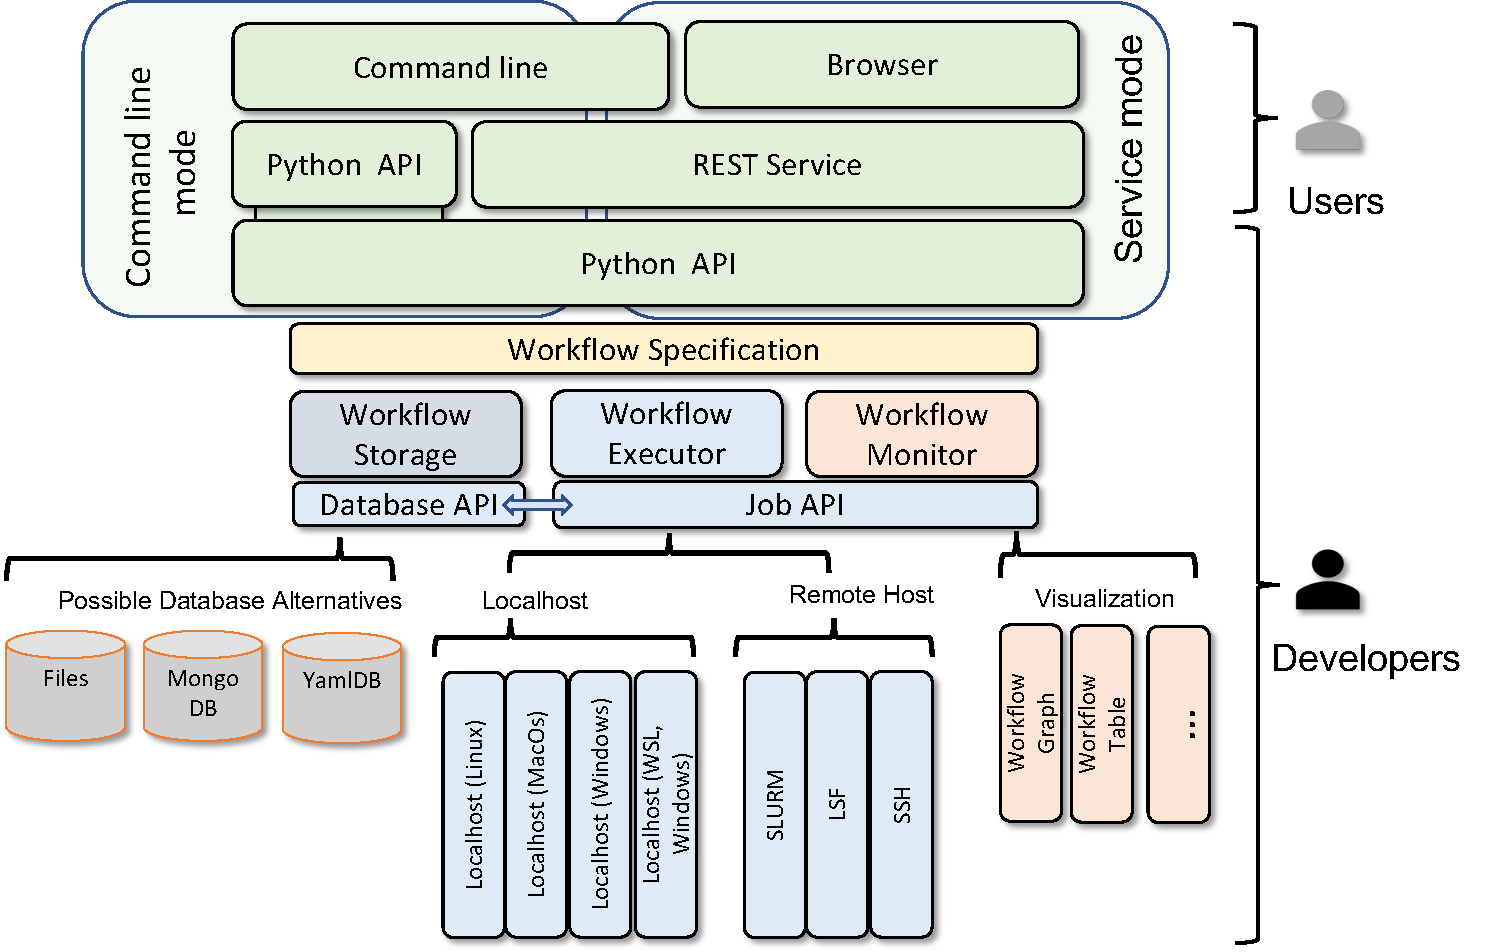
\includegraphics[width=1.0\columnwidth]{images/cloudmesh-cc-arch.pdf}
\caption{Architecture of the Framework}\label{fig:arch}
\end{figure}

The framework is based on a layered architecture so that it can be improved
and expanded on at each layer. We distinguish two kinds of users---developers 
and end users---that define their workflows to run on
computing resources. For the end user, we provide a command line and a
very simple browser interface. Simplicity is important as it does not
require spending exorbitant amounts of time to learn how to use the
workflow framework. To support developers, we have designed a minimal
Python API that is also used to implement a REST Service.  Currently,
the REST Service is supposed to run on the client, but a service
deployment could also be conducted while assuring that proper
authentication and authorization are used. This is easily possible as
we use a well-known REST service framework (FastAPI) that can
integrate with common security frameworks to secure services. The API,
workflow specification, command line interface, and browser are 
well-documented with the help of Sphinx and OpenAPI.

The workflow specification plays an important role in not only
defining a workflow but also keeping the status of a currently
executed workflow. Here we have completely separated the status of the
workflow and synchronized the state of the workflow with pull requests
to the service that executes the computation. This allows the system
to be shut down at any time while the running jobs are completely
independent of the client application accessing the state. Thus, the
client appears to be stateless and fetches the state of the submitted
jobs on demand. It will return the latest state found on the job
execution services.

The workflows are defined with human-readable YAML. The workflow is stored in a
database that can be implemented using a variety of backends, such as
YamlDB, which is file-based and provides the easiest integration.

As we use a YAML file to represent the status of the workflow, it is
easy to create monitoring components (for example, as part of a Web
browser). Various sophisticated graph display frameworks could be
used. For now, we have simply exposed the graph in table format using
DataTables.net and the graph as an SVG file while leveraging Graphviz.

One of the most important parts of the framework is how we manage jobs
and monitor their status. For this, we have introduced an abstract job
class that is integrated into our workflow class. The job class can
define jobs, start them, and cancel them, to name only the most
important management methods. However, each job defines a status file
in which the actual progress of the job is recorded. This status file
is managed on the compute resource where the job is run and is queried
on demand to return the status to the client. This way, the status of
all jobs can be monitored. As our goal is not to run jobs that execute
in milliseconds but rather in the second range, such status reporting
and propagation is well-suited for us. We have defined a special
status progress update specification that is universally
applicable. These jobs can be bash scripts, Python scripts, Jupyter
notebooks, or Slurm scripts.

Workflows are compilations of jobs to be run on nodes. These workflows
report information on the status of jobs as they are run, whether
locally or remotely. These types of jobs can be mixed with others into
a single workflow. This allows us, as already mentioned, to view the
progress of a workflow as it is being run in quasi-realtime.  The
workflow can be monitored as a graph or a data table. These interfaces
report the statuses of the jobs. Additionally, the order in which the
jobs are run can be specified, enabling prerequisite jobs and the
segmentation of a workflow.

To address the requirement of simplicity, the overall code is less
than 3600 lines of code, with additional 2600 lines for extensive test
cases.

The framework is managed as an open-source repository in GitHub and
uses Python as the implementation language. The code is compatible
with Windows, macOS, and Linux.

It is crucial to note that, in addition to this task parallel approach
allowing us to integrate hybrid resources controlled by the user, we
also have the experiment executer which we describe in more detail in
Section~\ref{sec:cloudmesh-sbatch}.

We will first focus on our ability to specify task parallel workflows.

\section{Specifying Task-based Workflows}
\label{sec:task-workflow}

The workflow definition for cloudmesh is rather simple and intuitive.
An example is provided in Figure~\ref{fig:workflow-example}. Here, a
DAG with three nodes is specified ($start \rightarrow f\!etch\!-\!data
\rightarrow compute \rightarrow analyze \rightarrow end$). In this
example the
workflow executes three scripts
(test-[fetch-data,compute,analyze].sh). It contains a specific start
and end node. This is a typical use pattern for DL-related analysis tasks. Dependencies can easily be specified in human-readable format while using the node name. The nodes contain easy-to-manage information such as the name of the node and a label that is used to print the node's progress. The label may contain variables that can be custom designed and added to the workflow. Default variables that are frequently used include {\em name}, {\em progress}, and {\em now}. Nodes can also have a type indication if it represents
a Python, sh,
Jupyter, or Slurm task. Additionally, for Python, one can specify the virtual environment with venv, allowing multiple venvs to be used in the same workflow.

The node attributes are listed and summarized 
in
Table~\ref{tab:node-attributes}, while details about the labels are listed in Table \ref{fig:labels-list}. As the labels and styling are simple to use but have a powerful impact on the display of the workflow, we document some of its features in the next sections.

\begin{figure}[htb]
{\scriptsize
\begin{lstlisting}[breaklines=true]
(*\bfseries workflow:*)
  (*\bfseries nodes:*)
    start:
       name: start
    fetch-data:
       name: fetch-data
       user: gregor
       host: localhost
       kind: local
       status: ready
       label: '{name}\nprogress={progress}'
       script: test-fetch-data.sh
    compute:
       name: compute
       user: gregor
       host: localhost
       kind: local
       status: ready
       label: '{name}\nprogress={progress}'
       script: test-compute.sh
    analyze:
      name: analyze
      user: gregor
      host: localhost
      kind: local
      status: ready
      label: '{name}\nprogress={progress}'
      script: test-analyze.sh
    end:
       name: end
  (*\bfseries dependencies:*)
    - start,fetch-data,compute,analyze,end
\end{lstlisting}}
\caption{Workflow YAML Configuration file.}\label{fig:workflow-example}
\label{fig:yaml-file}
\end{figure}

\begin{table}[htb]
\centering
\caption{Node attributes.}\label{tab:node-attributes}


{\scriptsize
\begin{tabular}{|l|p{6cm}|}
\hline
{\bf Attribute} & {\bf Description} \\
\hline
\hline
name &  A unique name of the job, must be the same as defined in the : line \\
\hline
user &  The username for the host \\
\hline
host &  The hostname \\
\hline
kind &  The kind of the job, which can be local, ssh, wsl, or slurm  \\
\hline
status &  The status of the job in integer value between 0 and 100 \\
\hline
label &  A custom-designed label \\
\hline
script &  The script name to be executed \\
\hline
\end{tabular}
}

\bigskip

\caption{List of possible labels for nodes on the graph.}
\label{fig:labels-list}

{\scriptsize
  \begin{tabular}{|p{3.5cm}|p{4cm}|}
    \hline
    {\bf Name} & {\bf Description} \\
    \hline
    \hline
    progress &  progress of job from 0-100 \\
    \hline
    now & current time \\
    \hline
    now.\verb|%Y%m%d,%H--%M--%S| &
   now in particular format (this can be used for other times as well) \\
    \hline
    created & time when workflow was created \\
    \hline
    t0.\verb|%Y%m%d,%H--%M--%S| &  workflow start time \\
    \hline
    t1.\verb|%Y%m%d,%H--%M--%S| & workflow end time \\
    \hline
    dt0.\verb|%Y%m%d,%H--%M--%S| & elapsed time since workflow began \\
    \hline
    dt1.\verb|%Y%m%d,%H--%M--%S| & total time of workflow once complete \\
    \hline
    tstart.\verb|%Y%m%d,%H--%M--%S| & job start time \\
    \hline
    tend.\verb|%Y%m%d,%H--%M--%S| & job end time \\
    \hline
    modified.\verb|%Y%m%d,%H--%M--%S| & job modified time \\
    \hline
    os. & operating system environment variable (like os.HOME) \\
    \hline
    cm. & cloudmesh variable that is read from \verb|cms set| \\
    \hline
\end{tabular}
}

\end{table}

\subsection{Node labels}

One particular useful attribute is that of a label. If no label is
used, the name of the node is used as the label. However, if a label
is specified, one can use attribute names and timers to create
labels with implicit state information. This is done by introducing
variables through curly braces. This is of special interest as our DL benchmarks may run a long time and we may want to monitor the progress. 
Table~\ref{fig:labels-list} shows the many useful time-based names one can use in a label. When such a name is used, it can also specify the format of the timer as indicated in an example in the table that shows the default format.

\subsection{Shapes and Styles}

Presently, we use Graphviz \cite{www-graphviz} for rendering the workflow. Thus we also integrated the ability to define attributes provided by Graphviz such as shapes and styles. The full palette of Graphviz features in regard to shapes and styles is supported.

\subsection{Reporting Progress}\label{reporting-progress}

When running jobs inside a Cloudmesh workflow, the called scripts can use a standard format provided by 
{\em cloudmesh.progress} to notify the user and the
backend client monitoring system. This is available in Python, shell, and any other framework as it can be implemented using a write to STDOUT. Such progress is augmented by an integer which indicates 0-100\% progress.
A trivial example encapsulating a machine learning program is shown next.

% {\scriptsize
\begin{lstlisting}[style=sh]
  echo "# cloudmesh status=running progress=1 pid=$$"
  singularity exec --nv ./cloudmask.sif cloudmask.py --config config.yaml 
  echo "# cloudmesh status=done progress=100 pid=$$"
\end{lstlisting}
% }

For Python scripts and Jupyter notebooks, a built-in function is provided as shown next.

% {\scriptsize
\begin{lstlisting}[style=python]
  from cloudmesh.common.StopWatch import progress
  filename = './cloudmesh-log-file.log'
  Stopwatch.start("total")
  progress(progress=1, filename=filename)
  # ... execute your analysis here ...
  progress(progress=100, filename=filename)
  Stopwatch.end("total")
  Stopwatch.benchmark() # prints the benchmark results
\end{lstlisting}
% }

Obviously, such progress can be embedded in tools such as tqdm to automatize the logging and help trivial integration with the sophisticated Python ecosystem.

\subsection{Generating Progress Image as Graph}

The framework has a built-in capability to visualize and export the progress of the
workflow in a DAG.

In Figure~\ref{fig:workflow-process}, we depict a simple example
of a workflow that shows the progression of the status over time. Such simple visualization naturally helps to communicate the status and showcases it in the context of the entire workflow. This is often far superior to just monitoring log entries in a file.

\begin{figure}[htb]
\resizebox{1.0\columnwidth}{!}{
\begin{minipage}[b]{0.18\textwidth}
Definition and start \\
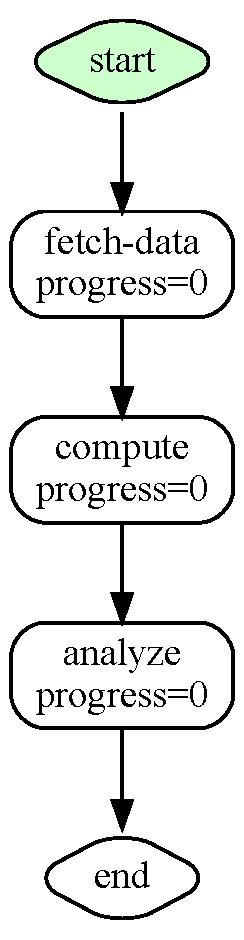
\includegraphics[height=9cm]{images/workflow-example-1.pdf}
\end{minipage} \ \
\begin{minipage}[b]{0.18\textwidth}
Running 1st task \\
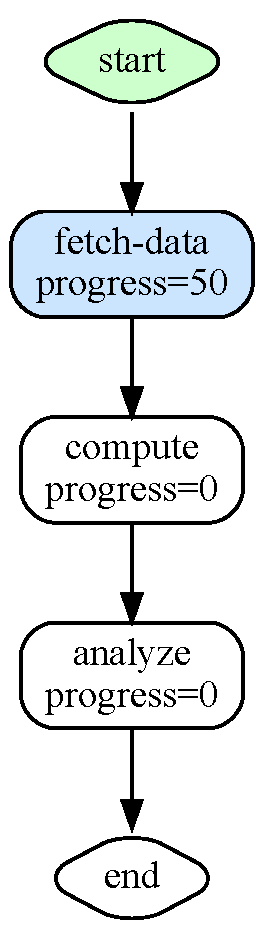
\includegraphics[height=9cm]{images/workflow-example-1.5.pdf} 
\end{minipage} \ \
\begin{minipage}[b]{0.18\textwidth}
Complete 1st task \\
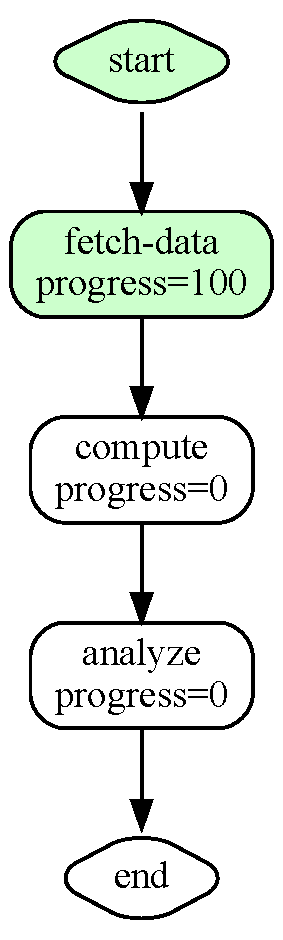
\includegraphics[height=9cm]{images/workflow-example-2.pdf}
\end{minipage} \ \
\begin{minipage}[b]{0.18\textwidth}
Complete 2nd task \\
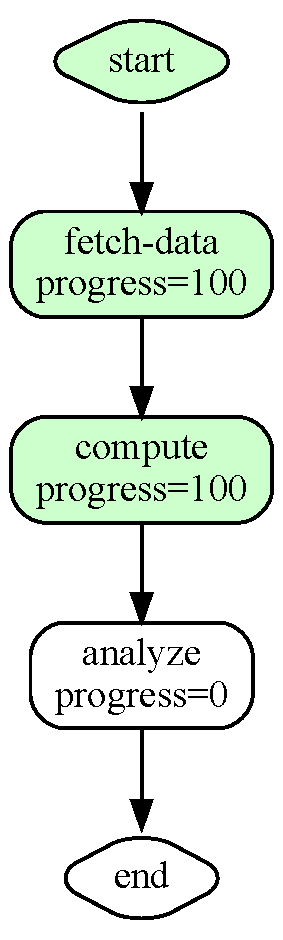
\includegraphics[height=9cm]{images/workflow-example-3.pdf}
\end{minipage} \ \
\begin{minipage}[b]{0.18\textwidth}
Complete workflow \\
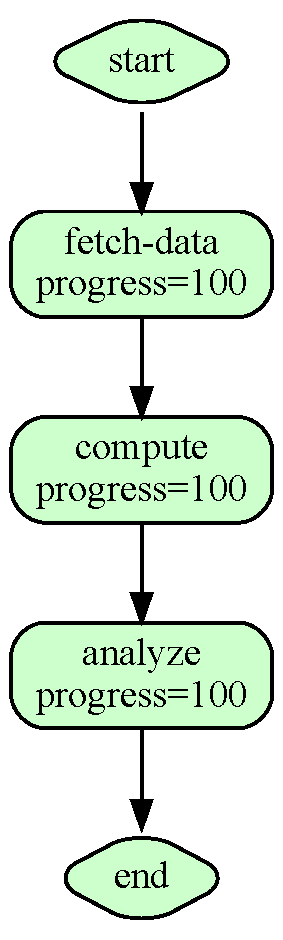
\includegraphics[height=9cm]{images/workflow-example-5.pdf}
\end{minipage} 
}
\caption{The gradual process of a simple workflow.}\label{fig:workflow-process}
\end{figure}


\section{Cloudmesh-cc Interfaces}
\label{sec:cloudmesh-cc-interfaces}

In this section, we explain the various ways of interfacing with the workflow which is distributed in a Python package 
{\em cloudmesh-cc} that includes all but the lower level of our design (see Figure~\ref{fig:arch} and the experiment executor which is implemented in a package called {\em cloudmesh-sbatch}). Interfaces to compute resources are, by design, able to be added via simple pip installs and (once installed through dynamic loading) integrated into the cloudmesh framework instantiation.

It is important to note that we also have a {\em command line mode} that interfaces directly with the backends while not requiring a service. All features are available as Python API. In addition, we have used this API to implement a {\em service}, allowing us to stand up a REST service and a GUI that can be accessed through a Web browser.
Please note that the service mode can also be accessed through the command line
in a terminal and native tools to display the workflow. 
We will now discuss these interfaces in more detail and also showcase
how we can access them.
To support direct execution on the command line, we also provide a command line interface and leverage the cloudmesh command shell, enabling us to interact with the system from the cloudmesh shell on-demand. 

Hence, our work can be integrated into many other frameworks or tools, some of which are listed in the Related Research section. Details of these APIs go beyond the purpose of this document and are summarized in \cite{las-22-arxiv-workflow-cc}.

In addition to the aforementioned interfaces, we also provide a simple Web GUI interface that allows a workflow to be administered and monitored through the GUI. At this time, it contains all the needed functionality to execute and monitor a workflow through a Web browser.

Figure \ref{fig:table-view} shows the table view of a possible cloudmask workflow, while Figure \ref{fig:graph-view} shows the graph view. During execution, the information in the views will be automatically updated through server-sent events.


\begin{figure}[htb]
{\centering
  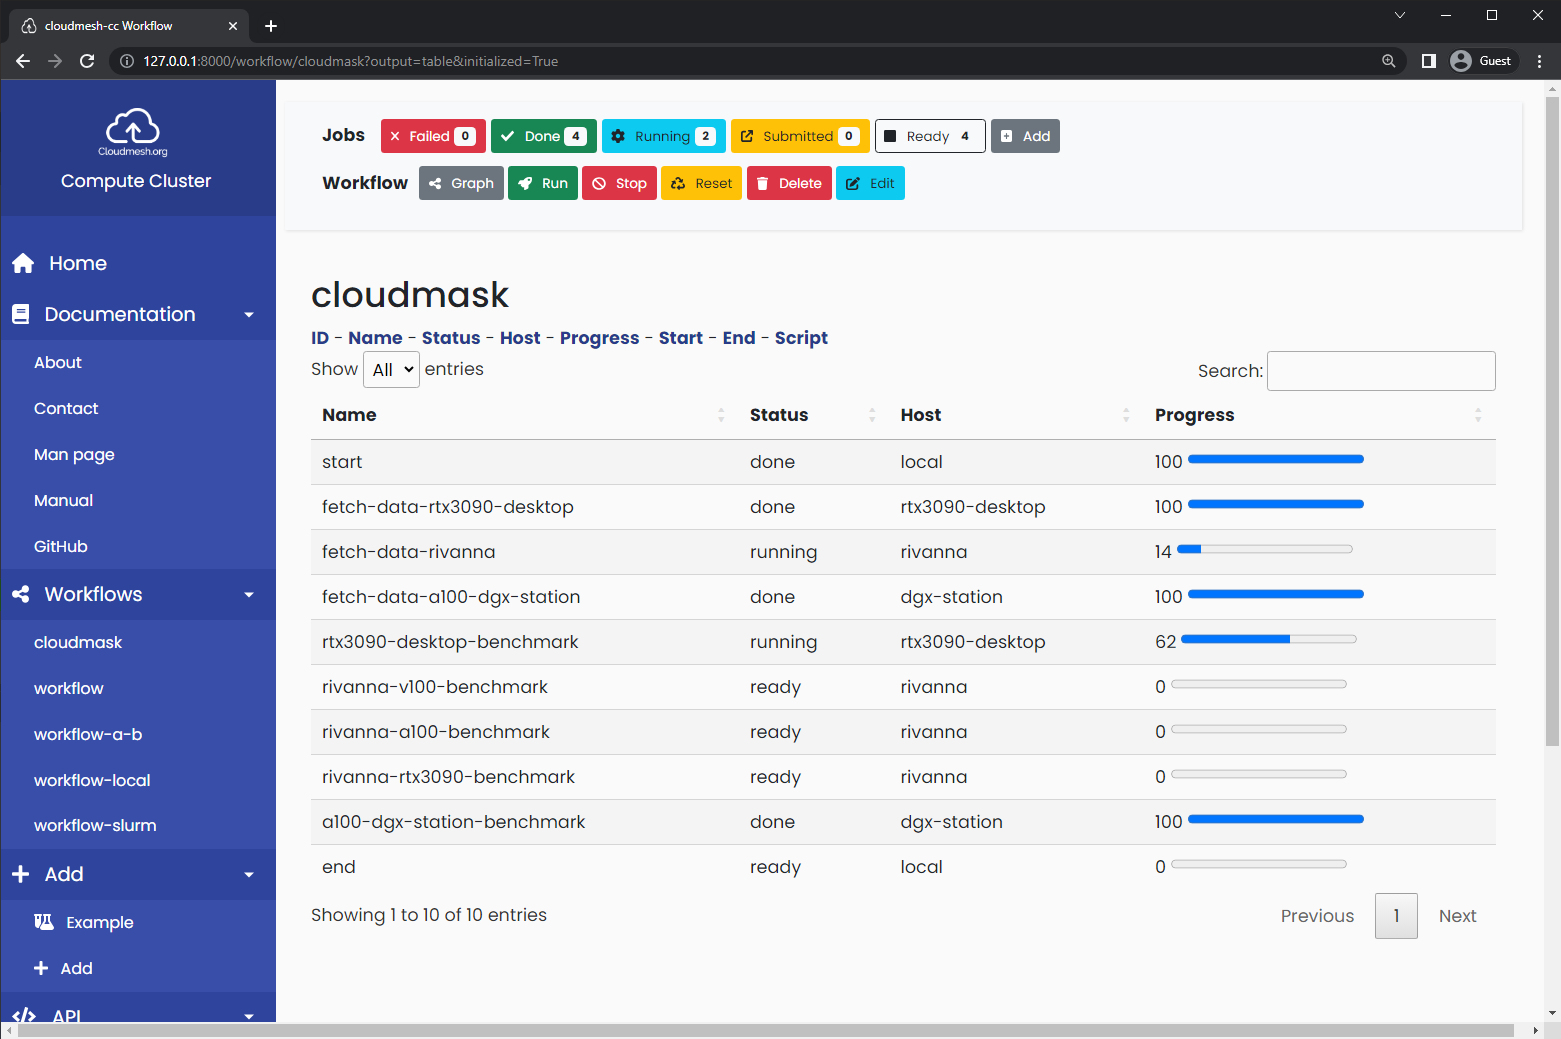
\includegraphics[width=1.0\columnwidth]{images/table-cloudmask-workflow.png}
}
\vspace{0.0cm}
\caption{Cloudmesh cc workflow table view.}
\label{fig:table-view}

\bigskip
{\centering
  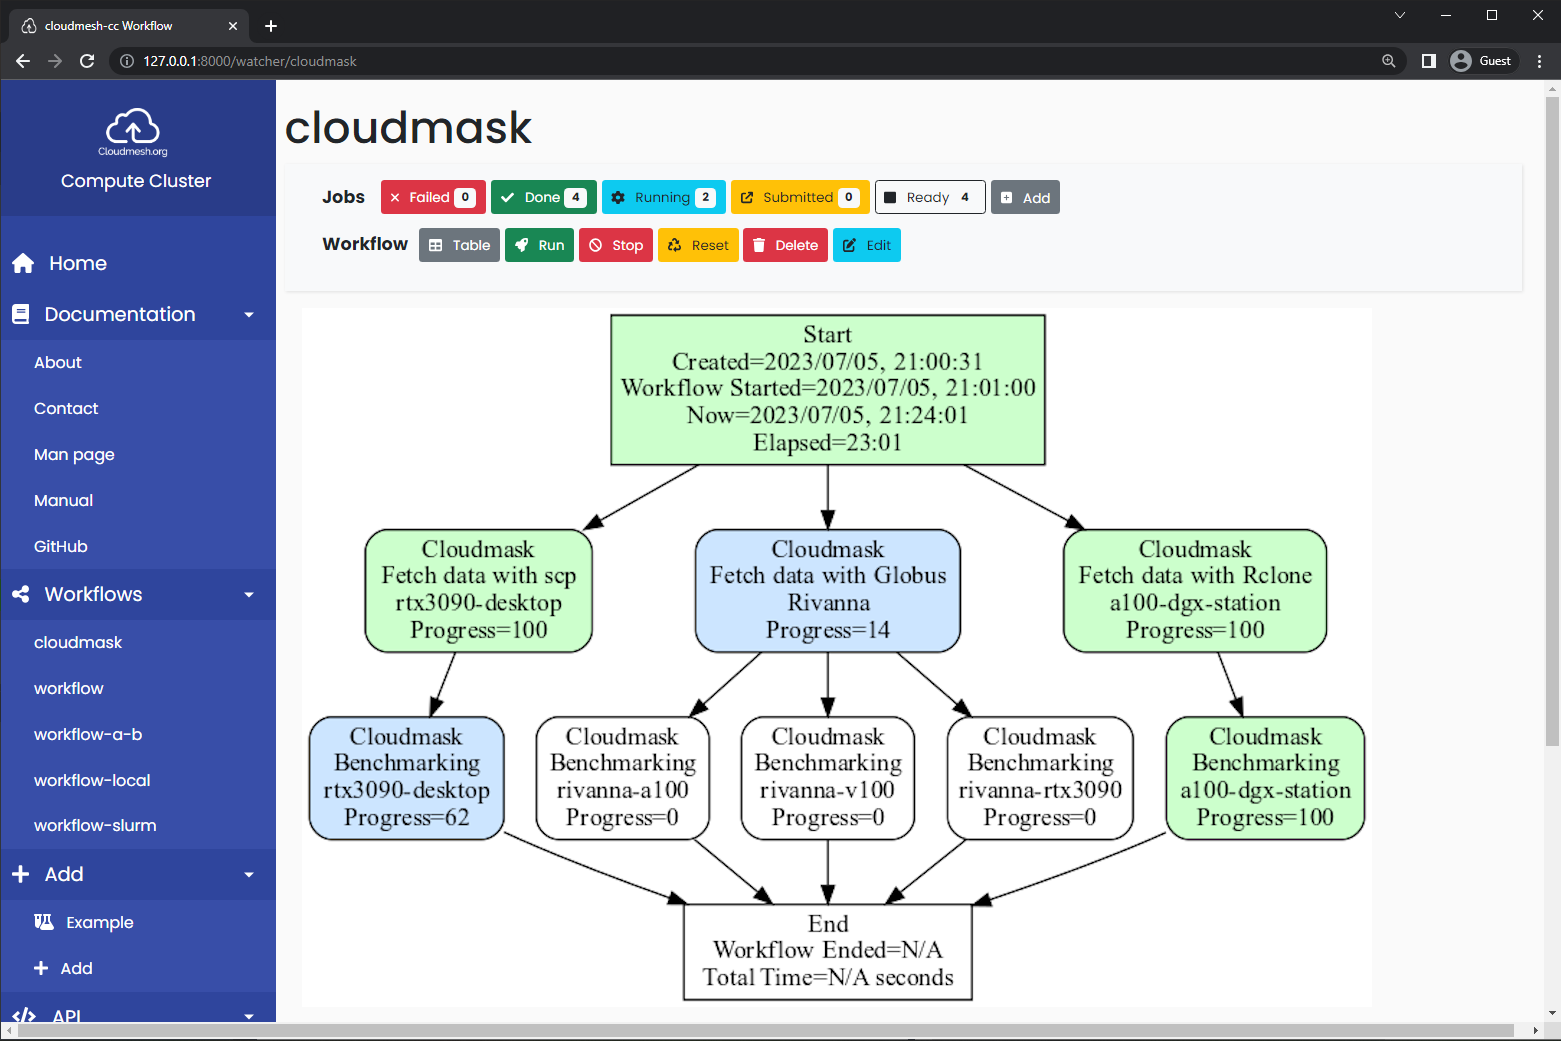
\includegraphics[width=1.0\columnwidth]{images/gui-cloudmask-workflow.png}
 }
\vspace{0.0cm}
 \caption{Cloudmesh cc workflow graph view.}
\label{fig:graph-view}

\end{figure}


\subsection{Cloudmesh-sbatch}
\label{sec:cloudmesh-sbatch}

\begin{figure}[htb]
    \centering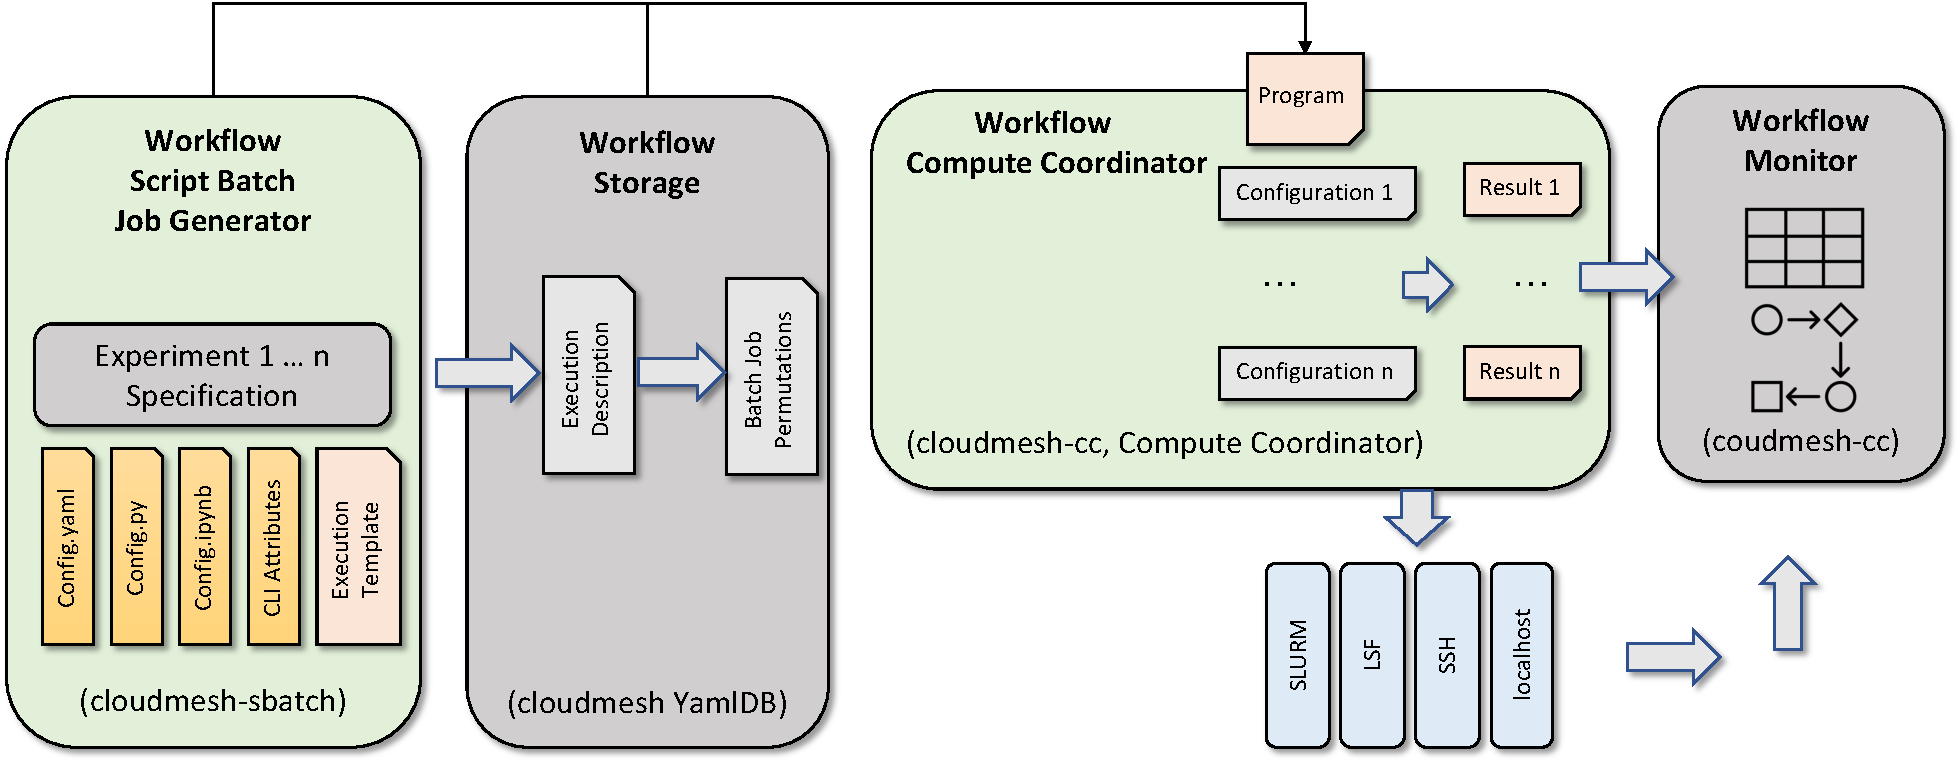
\includegraphics[width=1.0\columnwidth]{images/cloudmesh-sbatch-new}
    
    \caption{Experiment management workflow architecture design of cloudmesh-sbatch.}
    \label{fig:cc-2}

\end{figure}


\subsubsection{Specifying Experiment-Parameter-based Workflows}
\label{sec:workflow-sbatch}

In traditional machine learning workflows, hyperparameter tuning and configuration are key elements in assessing and optimizing the performance of models. However, scaling hyperparameters for highly parallel execution with heterogeneous hardware is complex.

Cloudmesh-sbatch is a hyperparameter and configuration management toolkit designed to address the generation of batch jobs with a consistent and configurable interface based on hyperparameter values across multiple development toolchains. They can also utilize the monitoring features as introduced in the previous section. One of its main functions is to create batch jobs based on parameterized job specifications and configuration files. As it is integrated with cloudmesh, it can leverage various queuing systems and submission commands through abstraction. Currently, we provide interfaces to Slurm, LSF, and ssh as these are the frameworks used on HPC and local resources we have access to. However, it would be possible to integrate others due to the extensible design of our framework.

The architecture of the cloudmesh-sbatch framework is depicted in Figure \ref{fig:cc-2} and demonstrates that it integrates with our previous cloudmesh-cc component.

Cloudmesh-sbatch generates a cartesian product (permutation) of hyperparameter to form independent {\it experiment} execution profiles, making it trivial to scale an experiment from one execution to thousands just by changing the configuration file. The resulting output provides a generated shell script that is custom created for the particular queuing system used on the resource. Within the configuration file for such a resource, we also use a YAML configuration file representing the specific hyperparameters. By managing many highly configurable jobs with cloudmesh-sbatch, the focus is placed on what hyperparameters to use for experiments and reducing the possibility of human error when running experiments over a range of hyperparameters. It is important to note that cloudmesh-sbatch is:

\begin{enumerate}
  \item using a unique directory for each experiment
  \item taking a parameter set from the cartesian product of the experiment parameters
  \item creating from a batch job template an instantiation of the template while replacing all variables from the configuration file and replacing the specific experiment parameters
  \item creating an instantiation of the configuration file while replacing all experiment parameters with the one for the current experiment.
\end{enumerate}

This is executed for all permutations of the experiment parameters. Through the creation of the unique experiment directory and the execution of the program in that directory with all output local to it, we have created implicitly a reproducible environment utilizing the files system hierarchy. Moreover, such output directories can be merged and results from multiple machines can be integrated as shown in Figure~\ref{fig:runtime-comp}.

To demonstrate how easy it is to use, we like to demonstrate a simple 
configuration file \verb|config.yaml| that includes specifications for where the data is located and which parameters are used in the application.

{\scriptsize
\begin{lstlisting}[breaklines=true]
    application:
        name: cloudmask
    data: "/scratch/{os.USER}/{application.name}"
    experiment:
        epoch: "1,30,60"
        gpu: "a100,v100"
        repeat: "1,2,3,4,5"
\end{lstlisting}
}

An example of a batch script that uses such a configuration is shown next.

{\scriptsize
\begin{lstlisting}[breaklines=true]
    #!/bin/bash

    #SBATCH --job-name={experiment.repeat}-{application.cloudmask}
    #SBATCH --nodes=1
    #SBATCH --gres=gpu:{experiment.gpu}:1
    #SBATCH --time=02:00:00
    #SBATCH --mem=64G
    #SBATCH -o {experiment.gpu}-{application.cloudmask}/{experiment.repeat}-%j.out
    #SBATCH -o {experiment.gpu}-{application.cloudmask}/{experiment.repeat}-%j.err
    #SBATCH --partition=bii-gpu
    #SBATCH --account=bii_dsc_community
    export USER_SCRATCH=/scratch/$USER
    cd USER_SCRATCH
    mkdir -p $USER_SCRATCH/{experiment.gpu}-{application.cloudmask}/%j.out
    nvidia-smi
    cms gpu watch --gpu=0 --delay=0.5 --dense > outputs/gpu0.log &
    python cloudmask.py --config config.yaml
    seff $SLURM_JOB_D
\end{lstlisting}
}

It is important to note that for each experiment, a custom batch file and configuration file is created that only includes the values for that particular experiment. In our example we also included an automated energy benchmark log observing intervall-based energy consumption on the GPUs leveraging cloudmesh-gpu.
To allow easy integration of parameters in YAML and shell scripts, we have provided a specific extension to YAML that allows us to fill in the value of a variable that is defined within a YAML file. The variables can easily be referred to with a dot notation in the templates. 

One can choose experiment parameters that best suit the application and benchmark.

While practically working with the system, we observed that students not using cloudmesh-sbatch often spend a significant amount of a semester on setting up a benchmark and replicating only a subset of the features that cloudmesh-sbatch provides. However, when a student uses it, we observed that the applications for which a template and configuration file has been designed reduced the on-ramp time to less than a day.

\section{Other Cloudmesh Features}
\label{sec:cloudmesh-other}

Cloudmesh comes with a sophisticated package management system,
allowing the integration of packages on demand targeting various providers
and capabilities, including a built-in command shell (not just only
a command line tool). Cloudmesh was first developed as a hybrid cloud
API, command line, and command shell framework. It provided AWS, Azure, Google, and OpenStack cloud interfaces for virtual
machine and data file services. It
is characterized by defining default templates for virtual machine
management on these clouds. Hence, it was possible to switch between clouds
with only a few commands and stage virtual machines on them.
% such as with the commands demonstrated in Figure~\ref{fig:cms}.


In addition, we have developed a package called GAS that addresses
the creation of analytics REST services from Python functions. This
package was developed to address the problem that integrating
deployment frameworks in the age of cloud computing is often out of
reach for domain experts. GAS is a simple framework allowing
non-experts to deploy and host services in the cloud. To avoid vendor
lock-in, it supports multiple vendors through cloudmesh vm
management~\cite{las21-gas}.

For benchmarking, we also have developed a special StopWatch library that measures times between named timers, as well as events. These timers are very convenient and output can be generated in a human-readable format as well as JSON, YAML, CSV, and MLLOG. Experience showed that the use of this library is for students simpler and more intuitive. However, as it produces also MLLog output automatically it can be used for any MLCommons application.  
 

\section{MLCommons Cloudmask Workflow}
\label{sec:cloudmask-workflow}

We have applied the workflow system to a number of applications. To provide an easy-to-use application, we have utilized MNIST and documented its use in our GitHub. However, here we demonstrate the use applied to the MLCommons Science Group Cloudmask application.


Cloudmask is a program that develops a model to classify sections of
satellite images as either containing clouds or clear skies by using
machine learning. This is beneficial for temperature measurement and
meteorology. Information regarding Cloudmask can be found on its
GitHub page~\cite{www-cloudmask}. One of our goals is to run
Cloudmask for benchmarking. As benchmarking Cloudmask requires
several phases and scripts, including a mixture of shell scripts and
Python scripts, leveraging cloudmesh-cc provides a much easier runtime
instead of manually issuing many commands at a terminal, especially when targeting hybrid multi-platform HPC machines with their own system dependencies. Hence, we have
created a sample workflow that runs a coordinated workflow across a
number of hybrid resources. This includes an HPC computer at the
University of Virginia called Rivanna, as well as two desktop
computers. This workflow can easily be adapted to include other
machines. In this particular workflow, we execute the benchmarks on a
number of different CUDA cards (see Figure~\ref{fig:runtime-comp}). For
Rivanna, the code also utilizes our cloudmesh-vpn component that
provides the ability to connect to the UVA VPN from Python, then
fetches the data and executes the various benchmarks once the data is
available.

\begin{comment}
\begin{figure*}[htb]
\centering
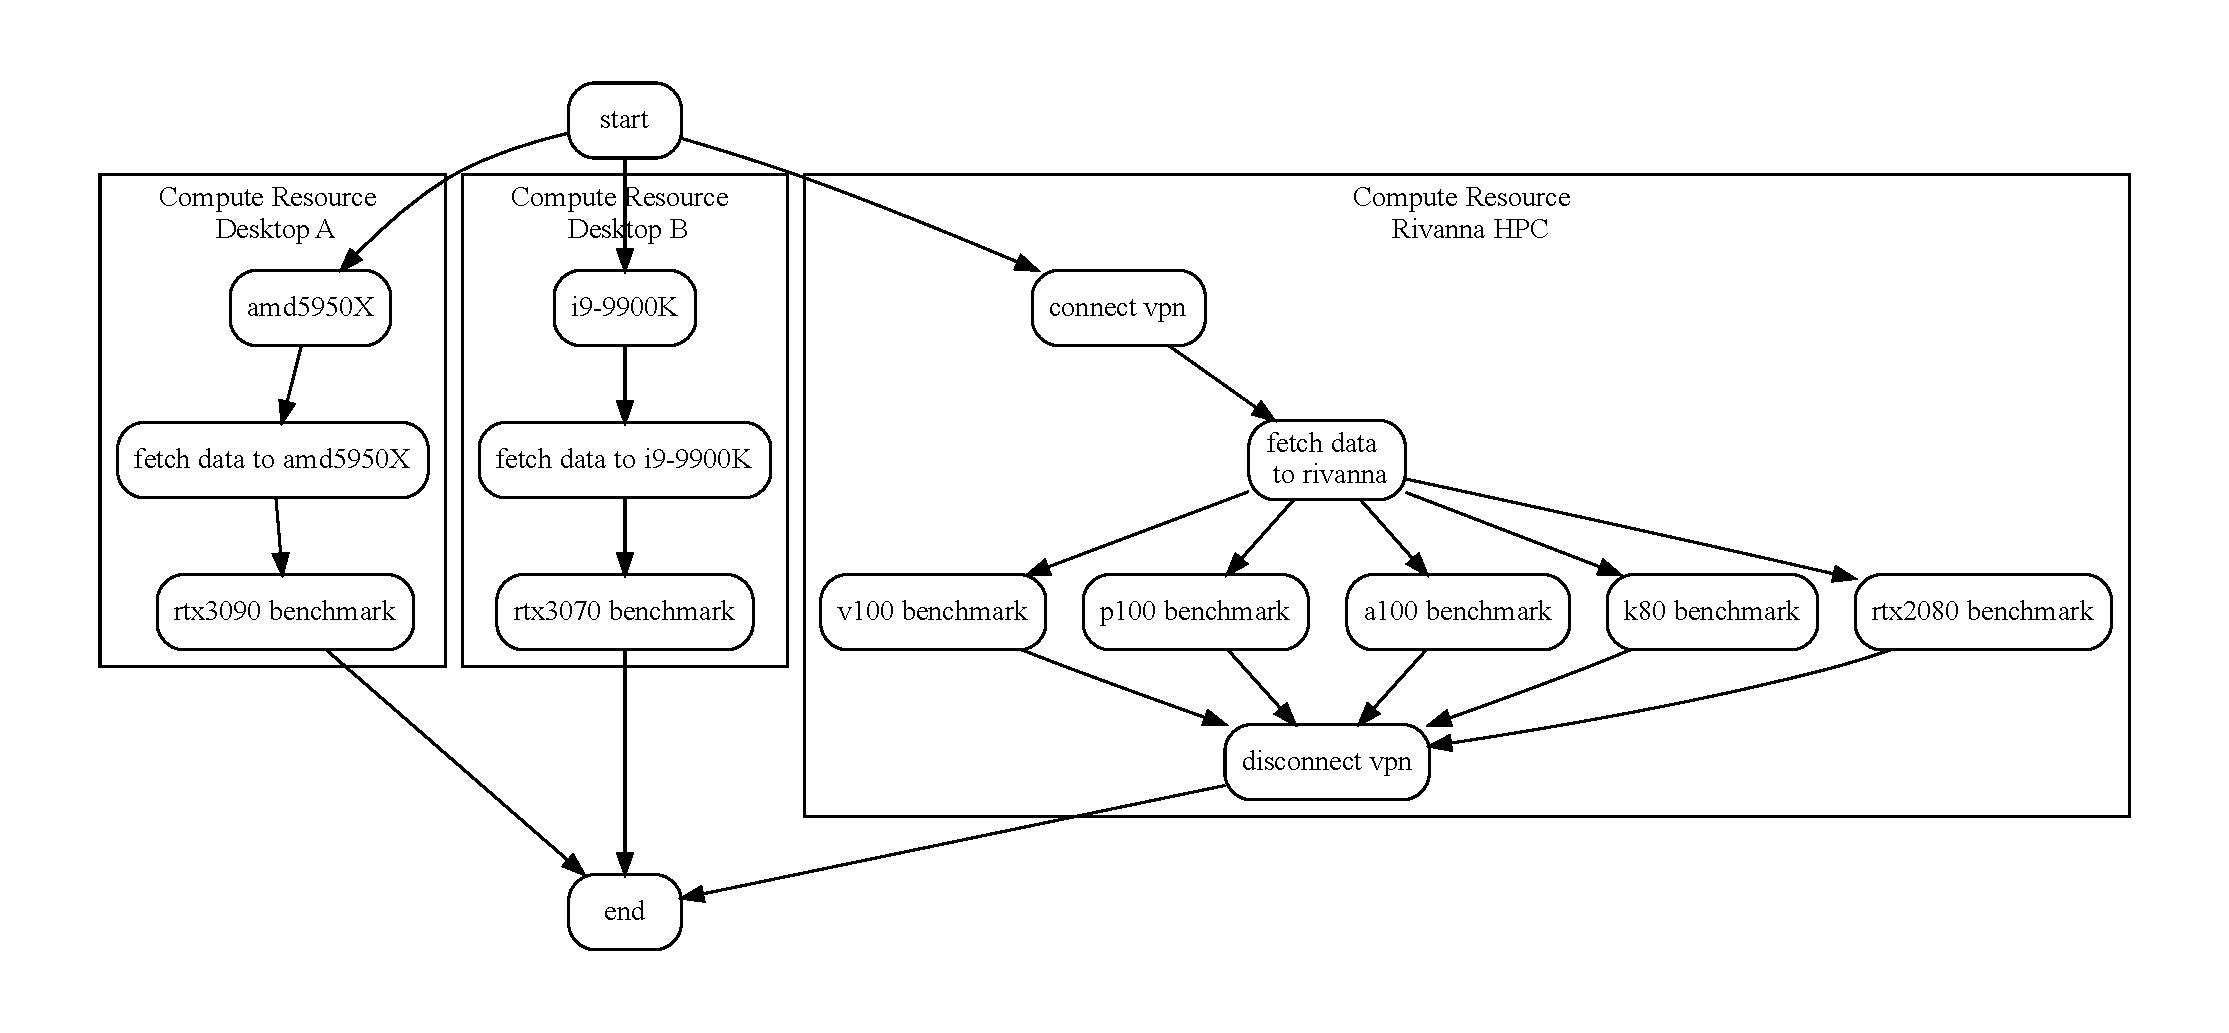
\includegraphics[width=0.75\textwidth]{images/cloudmask-wf.pdf}
%\vspace{-1cm}
\caption{Workflow for Cloudmask}\label{fig:cloudmaskwf}
\end{figure*}
\end{comment}

The workflow will take approximately 24 hours to run if resources are
available. The workflow iterates through five GPUs available on
Rivanna, including V100, P100, A100, K80, and RTX2080, and runs the
program three times on each GPU. Each run trains the model with 10,
30, and 50 epochs for benchmarking. Upon completing a run, the logs
and benchmarks are written into a results folder. 
In the following figures, we showcase a subset of the workflow 
to increase readability in this publication production of paper.

All results produced from the various machines can be agglomerated 
into a single analysis directory on which our Jupyter notebook can be run to produce customized outputs.

We showcase in Figures \ref{fig:runtime-comp}-\ref{fig:inf-acc-spectrum} selected templates that we include in our analysis script that can easily be adapted to other applications. It includes 
 benchmark comparisons of Cloudmask between graphics cards
(Figure~\ref{fig:runtime-comp}),
training history validation accuracy
(Figure~\ref{fig:train-hist-val-acc}),
training history validation loss
(Figure~\ref{fig:train-hist-val-loss}),
training history accuracy
(Figure~\ref{fig:train-hist-acc}),
training history loss
(Figure~\ref{fig:train-hist-loss}),
and more.

Additionally for this application, we integrated a custom analysis script that obtains differences in inference accuracy while aligning them with the various samples used for the inference as shown in the Figures titled
Inference accuracy (Figure~\ref{fig:inf-acc}) and
Inference accuracy over sample as a spectrum
(Figure~\ref{fig:inf-acc-spectrum}). The last two images from our workflow especially demonstrate that some training data perform poorly on our trained model for this application. Thus, a further improvement of the application is justified. Having our workflow and the templates as starting points will simplify research into this and other applications that utilize the framework. We are looking forward to an improved version of MLCube, which we will then integrate into this application and also utilize in our toolchain.



\begin{figure}[htb]
{\centering
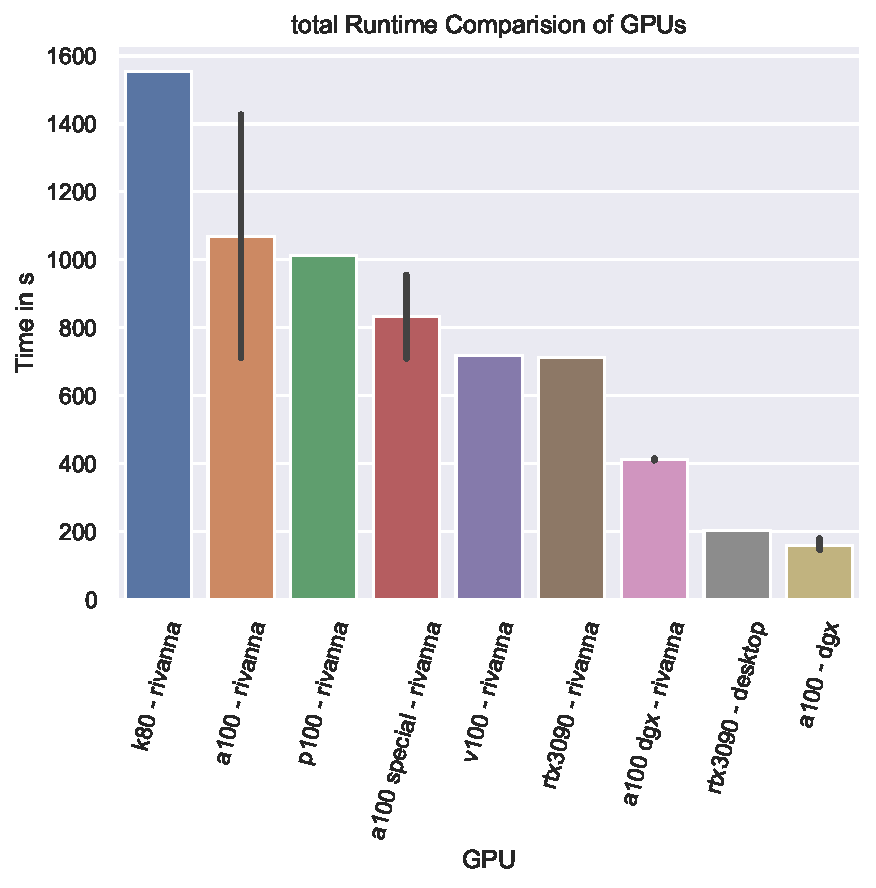
\includegraphics[width=1.0\columnwidth]{images/rivanna-comparision-epoch-1.pdf}
}
\caption{Runtime comparisons of Cloudmask between graphics cards}
\label{fig:runtime-comp}
\end{figure}

\begin{figure}[p]
{\centering
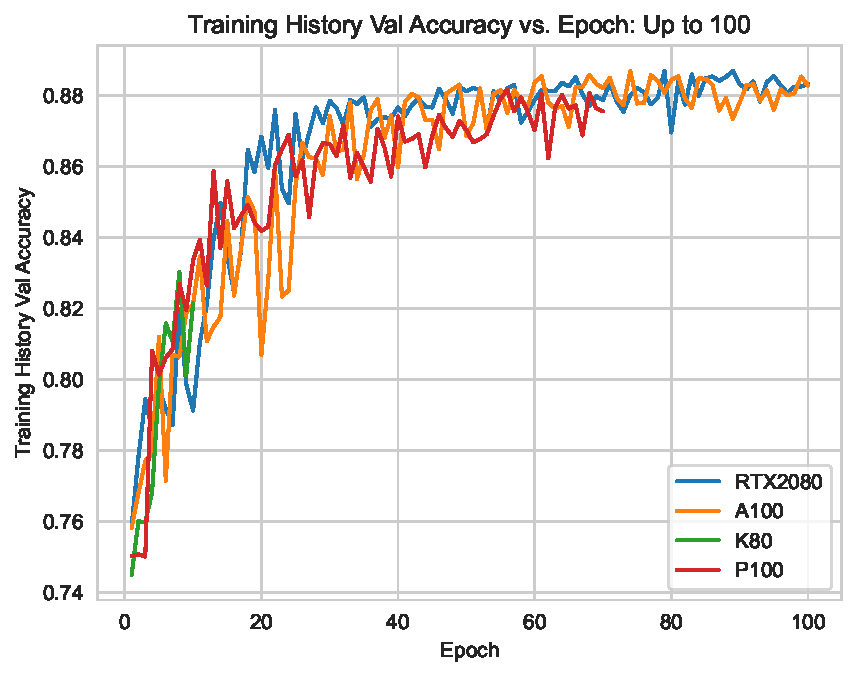
\includegraphics[width=1.0\columnwidth]{images/training-history-val_accuracy.pdf}
}
\vspace{-0.7cm}
\caption{Training history validation accuracy}
\label{fig:train-hist-val-acc}

\vspace{1cm}

{\centering
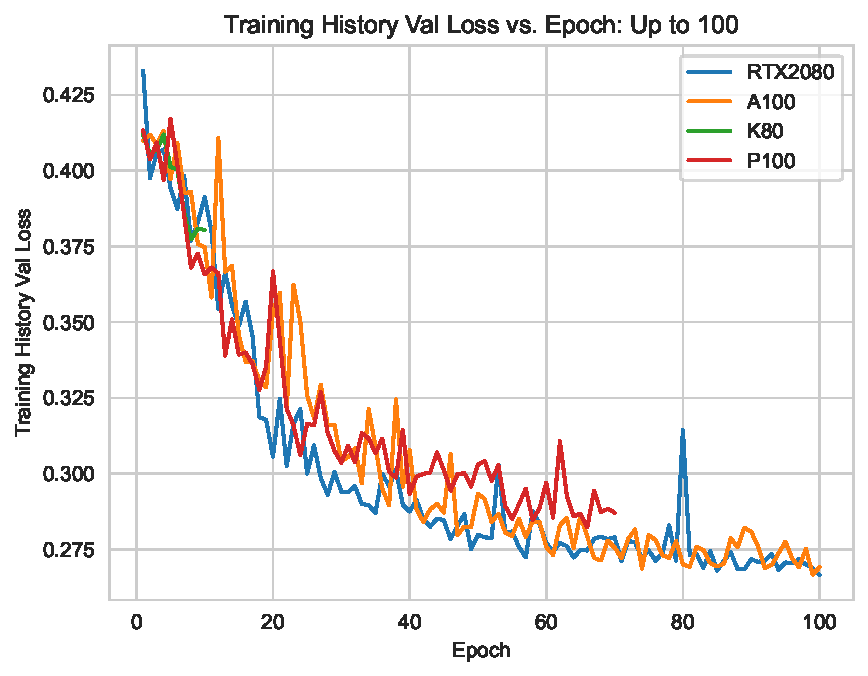
\includegraphics[width=1.0\columnwidth]{images/training-history-val_loss.pdf}
}
\vspace{-0.7cm}
\caption{Training history validation loss}
\label{fig:train-hist-val-loss}

\vspace{1cm}

{\centering
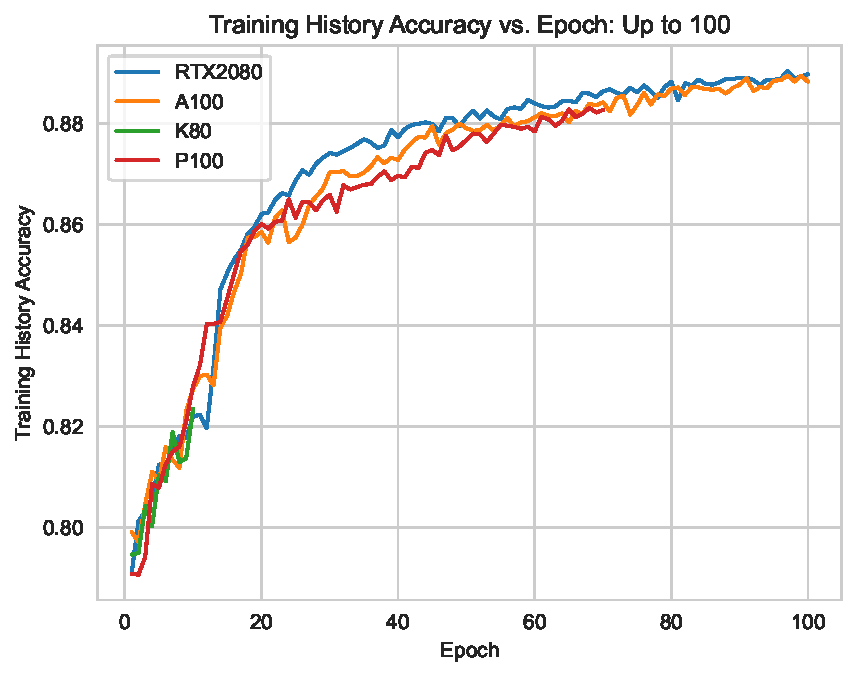
\includegraphics[width=1.0\columnwidth]{images/training-history-accuracy.pdf}
}
\vspace{-0.7cm}
\caption{Training history accuracy}
\label{fig:train-hist-acc}

\end{figure}

\begin{figure}[p]

{\centering
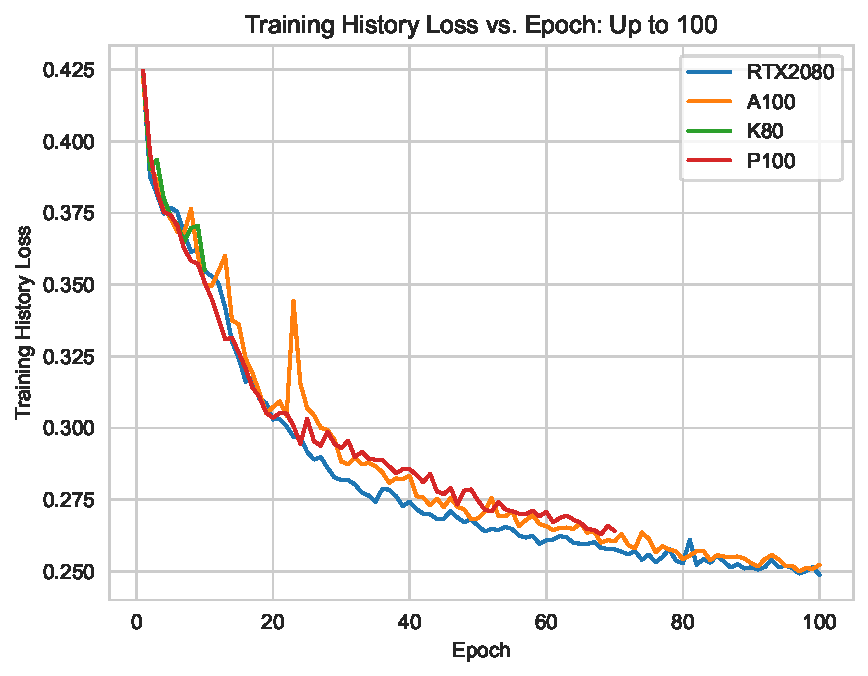
\includegraphics[width=1.0\columnwidth]{images/training-history-loss.pdf}
}
\vspace{-0.7cm}
\caption{Training history loss}\label{fig:train-hist-loss}

\vspace{1cm}

{\centering
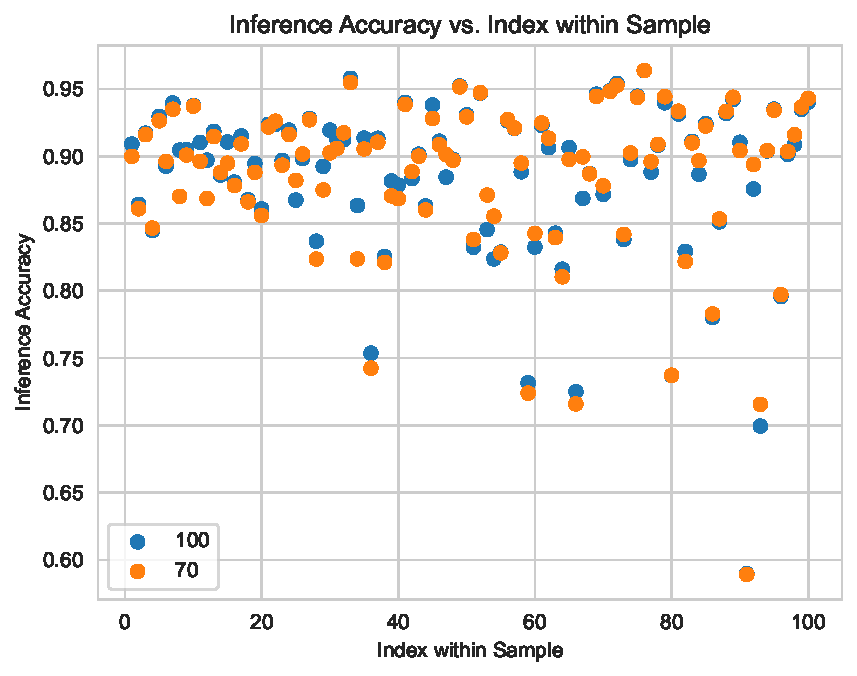
\includegraphics[width=1.0\columnwidth]{images/inference-accuracy.pdf}
}
\vspace{-0.7cm}
\caption{Inference accuracy}
\label{fig:inf-acc}

\vspace{1cm}

{\centering
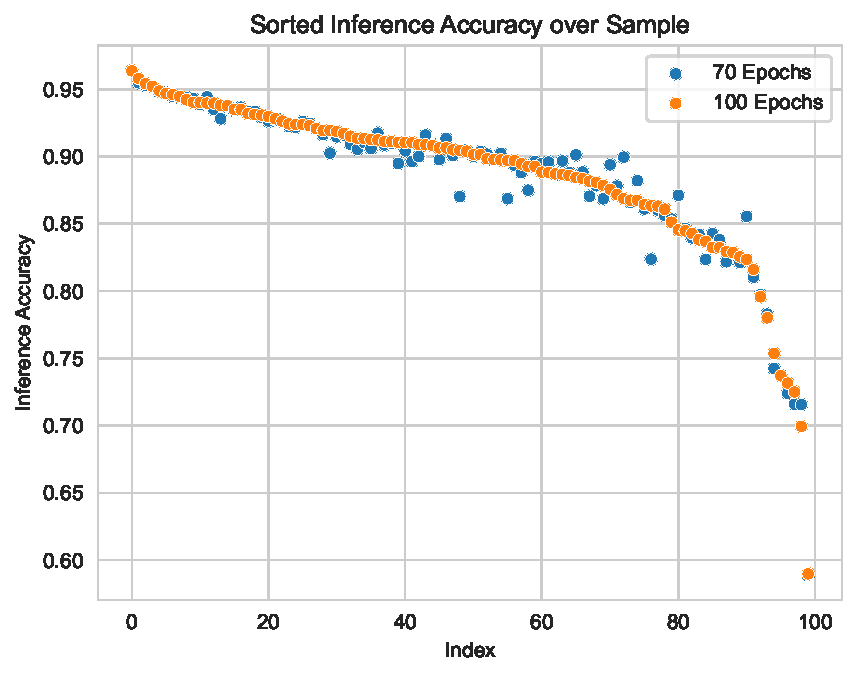
\includegraphics[width=1.0\columnwidth]{images/spectrum-inference-accuracy.pdf}
}
\vspace{-0.7cm}
\caption{Inference accuracy over sample as a spectrum.}
\label{fig:inf-acc-spectrum}
\end{figure}


\section{Conclusion}
\label{sec:conclusion}

We have designed and implemented a Hybrid Reusable Computational
Analytics Workflow Management with the help of the cloudmesh component
framework. The component added focuses on the management of workflows
for computational analytics tasks and jobs. The tasks can be executed
on remote resources via ssh and even access queuing systems such as
Slurm. In addition, we can integrate the current computer on which the
workflow is running. This can include operating systems such as Linux,
macOS, Windows, and even Windows Subsystem for Linux. Through
cloudmesh, access to a command line and a command shell is provided. A
simple API and a REST interface are provided. The framework also has
an elementary Web browser interface that allows visualizing the
execution of the workflow. It is important to know that the workflow
can be started on remote resources and is running completely
independently from the client tool once a task is started. This allows
a ``stateless'' model that can synchronize with the remotely started
jobs on demand. Hence, the framework is self-recovering in case of
network interruptions or power failure. Due to our experiences with
real (and many) infrastructure failures at the authors' locations, the
availability of such a workflow-guided system was
beneficial. Furthermore, the developed code is rather small and, in
contrast to other systems, is less complex. Hence, it is suitable for
educational aspects as it is used for master's and undergraduate level
research projects. The project has also been practically utilized
while generating benchmarks for the MLCommons Science Working Group
showcasing real-world applicability beyond a student research project.


\section*{Acknowledgment}

Work was in part funded by the NSF CyberTraining: CIC: CyberTraining for Students and Technologies from Generation Z with the award numbers 1829704 and 2200409 and NIST 60NANB21D151T.  The work was also funded by the Department of Energy under the grant Award No. DE-SC0023452. The work was conducted at the Biocomplexity Institute and Initiative at the University of Virginia.


\bibliographystyle{IEEEtran}

\bibliography{vonLaszewski-cloudmesh-cc}




\end{document}
\endinput
%%
%% End of file `sample-sigplan.tex'.

